% AnnData slot map: which stored array drives which AnnZarro view.
% The focused cell is a horizontal band, the focused gene a vertical band;
% wherever a band crosses an array is the slice one click fetches.
\begingroup
\definecolor{slcell}{HTML}{2A78D6}
\definecolor{slgene}{HTML}{EB6834}
\definecolor{sledge}{HTML}{8A8984}
\definecolor{slfill}{HTML}{F4F3EF}
\definecolor{slquiet}{HTML}{52514E}
\resizebox{\linewidth}{!}{%
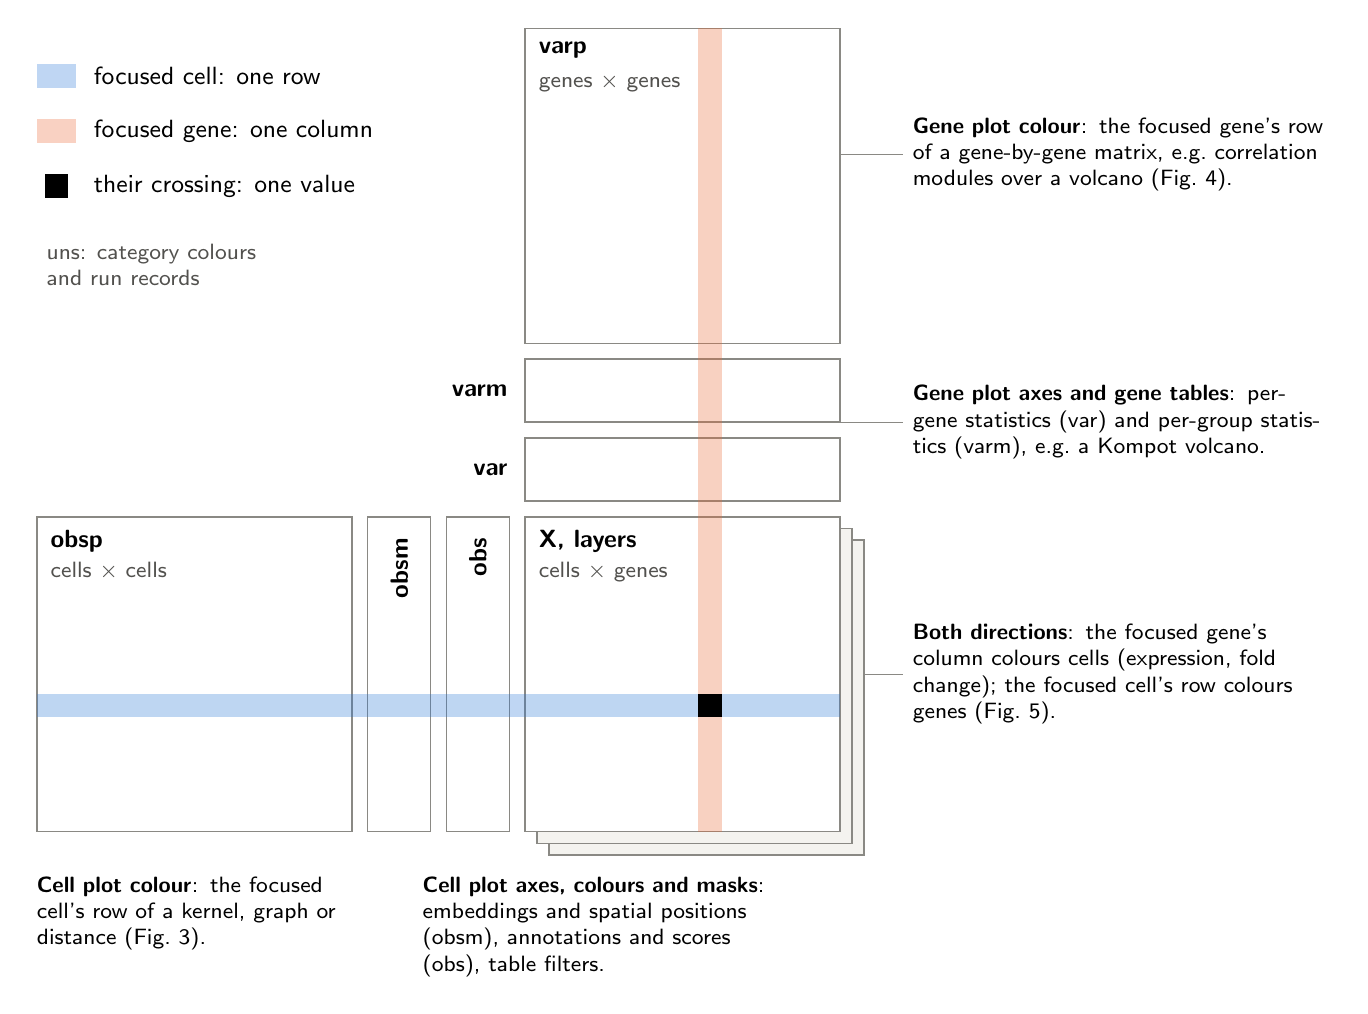
\begin{tikzpicture}[
  font=\sffamily\small,
  arr/.style={draw=sledge, line width=0.6pt, fill=white},
  slname/.style={font=\sffamily\small\bfseries, text=black},
  sldim/.style={font=\sffamily\footnotesize, text=slquiet},
  note/.style={font=\sffamily\footnotesize, text=black, align=left, text width=5.3cm, anchor=west},
  lead/.style={draw=sledge, line width=0.4pt},
]
  % layers peek out behind X
  \draw[arr, fill=slfill] (5.50,-0.30) rectangle (9.50,-4.30);
  \draw[arr, fill=slfill] (5.35,-0.15) rectangle (9.35,-4.15);
  % arrays
  \draw[arr] (5.2,0) rectangle (9.2,-4);        % X
  \draw[arr] (4.2,0) rectangle (5.0,-4);        % obs
  \draw[arr] (3.2,0) rectangle (4.0,-4);        % obsm
  \draw[arr] (-1.0,0) rectangle (3.0,-4);       % obsp
  \draw[arr] (5.2,1.0) rectangle (9.2,0.2);     % var
  \draw[arr] (5.2,2.0) rectangle (9.2,1.2);     % varm
  \draw[arr] (5.2,6.2) rectangle (9.2,2.2);     % varp

  % focus bands
  \fill[slcell, opacity=0.30] (-1.0,-2.25) rectangle (9.2,-2.55);
  \fill[slgene, opacity=0.30] (7.40,-4.0) rectangle (7.70,6.2);
  \fill[black] (7.40,-2.25) rectangle (7.70,-2.55);

  % array names
  \node[slname, anchor=north west] at (5.25,-0.05) {X, layers};
  \node[sldim,  anchor=north west] at (5.25,-0.45) {cells $\times$ genes};
  \node[slname, anchor=north west] at (-0.95,-0.05) {obsp};
  \node[sldim,  anchor=north west] at (-0.95,-0.45) {cells $\times$ cells};
  \node[slname, anchor=north west] at (5.25,6.15) {varp};
  \node[sldim,  anchor=north west] at (5.25,5.75) {genes $\times$ genes};
  \node[slname, anchor=east] at (5.1,0.6) {var};
  \node[slname, anchor=east] at (5.1,1.6) {varm};
  \node[slname, rotate=90, anchor=east] at (3.6,-0.15) {obsm};
  \node[slname, rotate=90, anchor=east] at (4.6,-0.15) {obs};

  % legend, top left
  \fill[slcell, opacity=0.30] (-1.0,5.75) rectangle (-0.5,5.45);
  \node[anchor=west] at (-0.4,5.6) {focused cell: one row};
  \fill[slgene, opacity=0.30] (-1.0,5.05) rectangle (-0.5,4.75);
  \node[anchor=west] at (-0.4,4.9) {focused gene: one column};
  \fill[black] (-0.90,4.35) rectangle (-0.60,4.05);
  \node[anchor=west] at (-0.4,4.2) {their crossing: one value};
  \node[sldim, anchor=west, align=left] at (-1.0,3.2) {uns: category colours\\and run records};

  % what each array drives
  \node[note] (nvarp) at (10.0,4.6) {\textbf{Gene plot colour}: the focused gene's row of a gene-by-gene matrix, e.g.\ correlation modules over a volcano (Fig.~4).};
  \node[note] (nvar) at (10.0,1.2) {\textbf{Gene plot axes and gene tables}: per-gene statistics (var) and per-group statistics (varm), e.g.\ a Kompot volcano.};
  \node[note] (nx) at (10.0,-2.0) {\textbf{Both directions}: the focused gene's column colours cells (expression, fold change); the focused cell's row colours genes (Fig.~5).};
  \draw[lead] (9.2,4.6) -- (nvarp.west);
  \draw[lead] (9.2,1.2) -- (nvar.west);
  \draw[lead] (9.5,-2.0) -- (nx.west);
  \node[note, anchor=north, text width=4.0cm] (nobsp) at (1.0,-4.45) {\textbf{Cell plot colour}: the focused cell's row of a kernel, graph or distance (Fig.~3).};
  \node[note, anchor=north, text width=4.4cm] (nobs) at (6.1,-4.45) {\textbf{Cell plot axes, colours and masks}: embeddings and spatial positions (obsm), annotations and scores (obs), table filters.};
\end{tikzpicture}}
\endgroup
